% -*- coding: UTF-8 -*-

\documentclass[UTF8,8pt,xcolor=dvipsnames]{beamer}

\usepackage{xeCJK}
\usepackage[utf8]{inputenc}

\usepackage{hyperref}
% \hypersetup{pdftex,colorlinks=true,allcolors=blue}
\usepackage{hypcap}

\usepackage{color}
\usepackage{xcolor}

\usepackage{amsmath}
\usepackage{mathtools}

\usepackage{blindtext}
\usepackage{enumitem}
\usepackage[ampersand]{easylist}
\usepackage{listings}
\usepackage{multicol}
\usepackage{fancybox}

\usepackage{tcolorbox}
% \usetikzlibrary{patterns}
% \tcbuselibrary{skins}
\tcbset{colback=yellow!5!white,colframe=yellow!75!black,boxrule=0.1mm}

\usepackage{indentfirst}

\usepackage{verbatim}
\usepackage{libertine}
\usepackage{graphicx}
\usepackage{framed}
\usepackage{pifont}
\usepackage[bottom]{footmisc}

\usepackage[normalem]{ulem}

\newcommand{\hl}{\bgroup\markoverwith
  {\textcolor{yellow}{\rule[-.5ex]{2pt}{2.5ex}}}\ULon}

\usepackage{makeidx}
\makeindex

\setlist{noitemsep}
%\usetheme{Warsaw}
%\usetheme{Szeged}
%\usetheme{Berkeley}
\usetheme{Hannover}
\usecolortheme{seahorse}

\AtBeginSection[]
{
    \begin{frame}
        \frametitle{目录}
        \tableofcontents[currentsection]
    \end{frame}
}

\newenvironment{myeasylist}[1]{
    \Activate
    \begin{tcolorbox}
    \begin{easylist}[#1]
} {
    \end{easylist}
    \end{tcolorbox}
    \Deactivate
}

\newenvironment{myslide}[1]{
    \begin{frame}[fragile]
    \frametitle{#1}
} {
    \end{frame}
}


%% ----------------- MAIN -------------------

\title{性能之巅}
\subtitle{SUZAKU性能优化之路}
\author{@DGJ}
\institute{北京大道云行科技有限公司}
\date{\today}

\begin{document}

\maketitle
% \tableofcontents

\section{架构}

\subsection{演进}

\begin{frame}[fragile]
    \frametitle{存储虚拟化}
    \begin{center}
    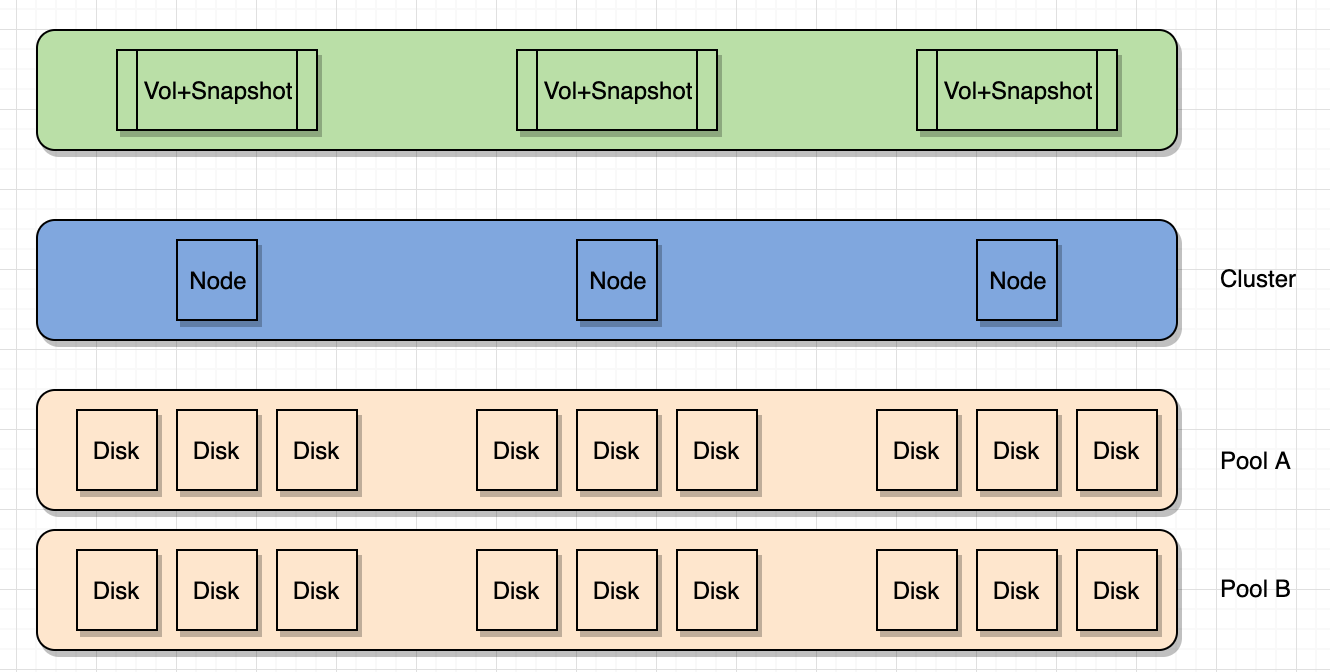
\includegraphics[width=0.8\textwidth]{../imgs/cluster-virt.png}
    \end{center}
\end{frame}

\begin{frame}[fragile]
    \frametitle{FusionStor的架构特点}
    \begin{myeasylist}{enumerate}
        & 元数据(非DHT)
        & 全用户态
        & core绑定 (PMD: polling mode driven)
        & Hugepage-based的内存管理
        & 直接访问裸盘(libaio/libnvme + KV)
        & 异步通信(TCP/RDMA)
        & 协议:iSCSI/iSER/NVMf
        & 编程模型:协程
    \end{myeasylist}
\end{frame}

\begin{frame}[fragile]
    \frametitle{从FusionStor到Suzaku之一}
    \begin{myeasylist}{enumerate}
        & 支持大卷
        & 单卷负载均衡
        & IO路径上的数据转发
        & 全局负载均衡(disk and core)
        & 元数据服务器MdCtl
            && 卷的元数据
            && chunk的副本信息
            && ROW快照的v2p映射
        & 更多信息记录在ETCD上
            && FS namespace
            && xattr
            && snapshot tree
    \end{myeasylist}
\end{frame}

\begin{frame}[fragile]
    \frametitle{从FusionStor到Suzaku之二}
    \begin{myeasylist}{enumerate}
        & 多进程:frctl、rangectl、bactl、mdctl?
        & get\_token
        & 网络连接模型 (all to all)
        & etcd采用了短连接
    \end{myeasylist}
\end{frame}

\begin{frame}[fragile]
    \frametitle{Universal Flash Planform}
    \begin{center}
        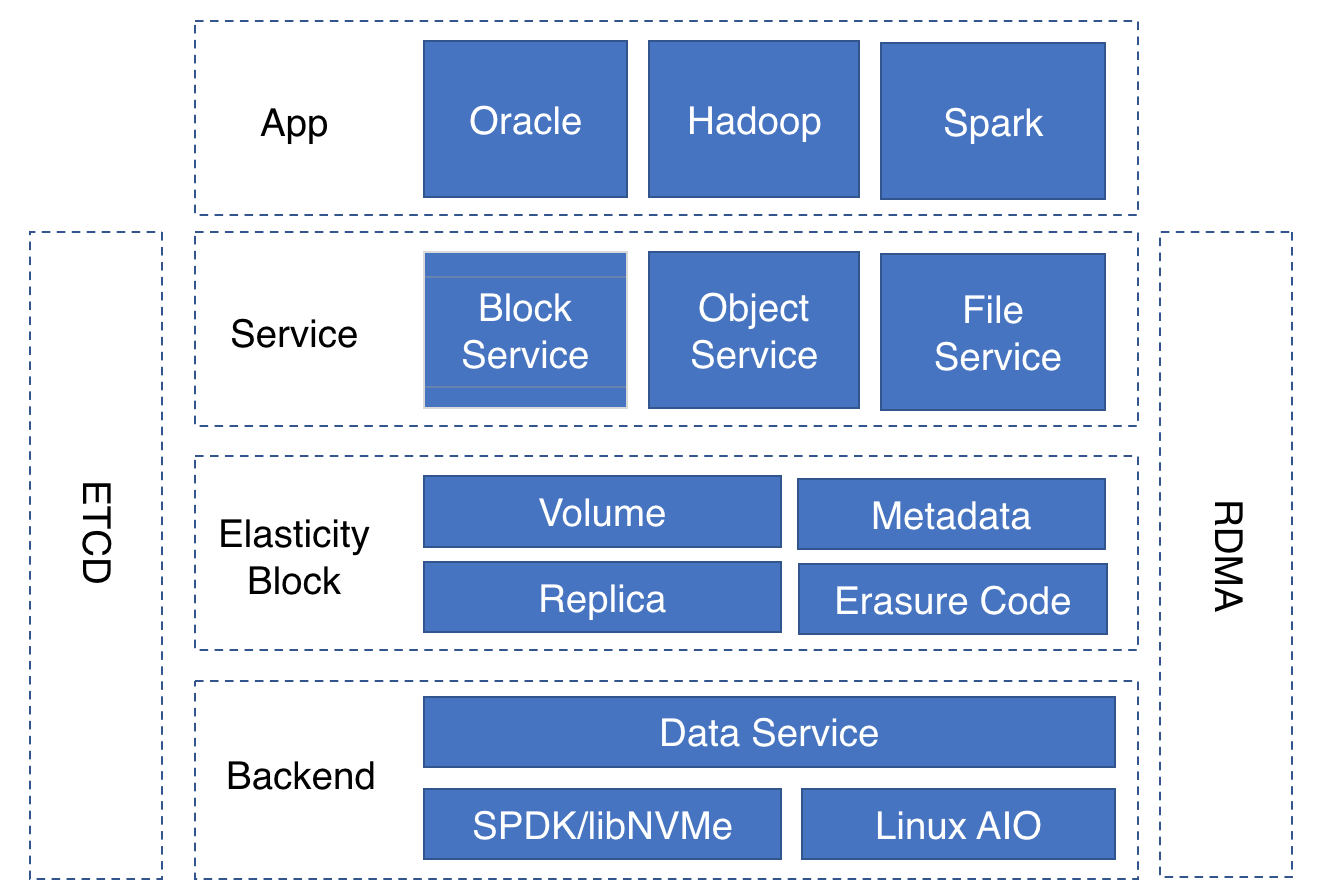
\includegraphics[width=0.6\textwidth]{../imgs/universal-flash.png}
    \end{center}
\end{frame}

\begin{frame}[fragile]
    \frametitle{操作系统}
    \begin{center}
        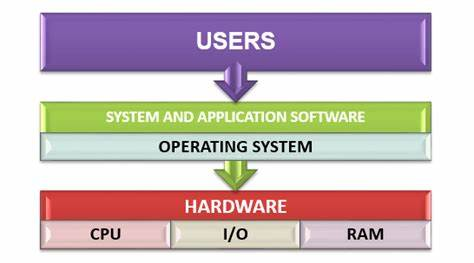
\includegraphics[width=0.5\textwidth]{../imgs/operating-system.jpeg}
    \end{center}
\end{frame}

\subsection{组件}

\begin{frame}[fragile]
    \frametitle{组件分解}
    \begin{columns}
        \begin{column}{0.5\textwidth}
            \begin{center}
                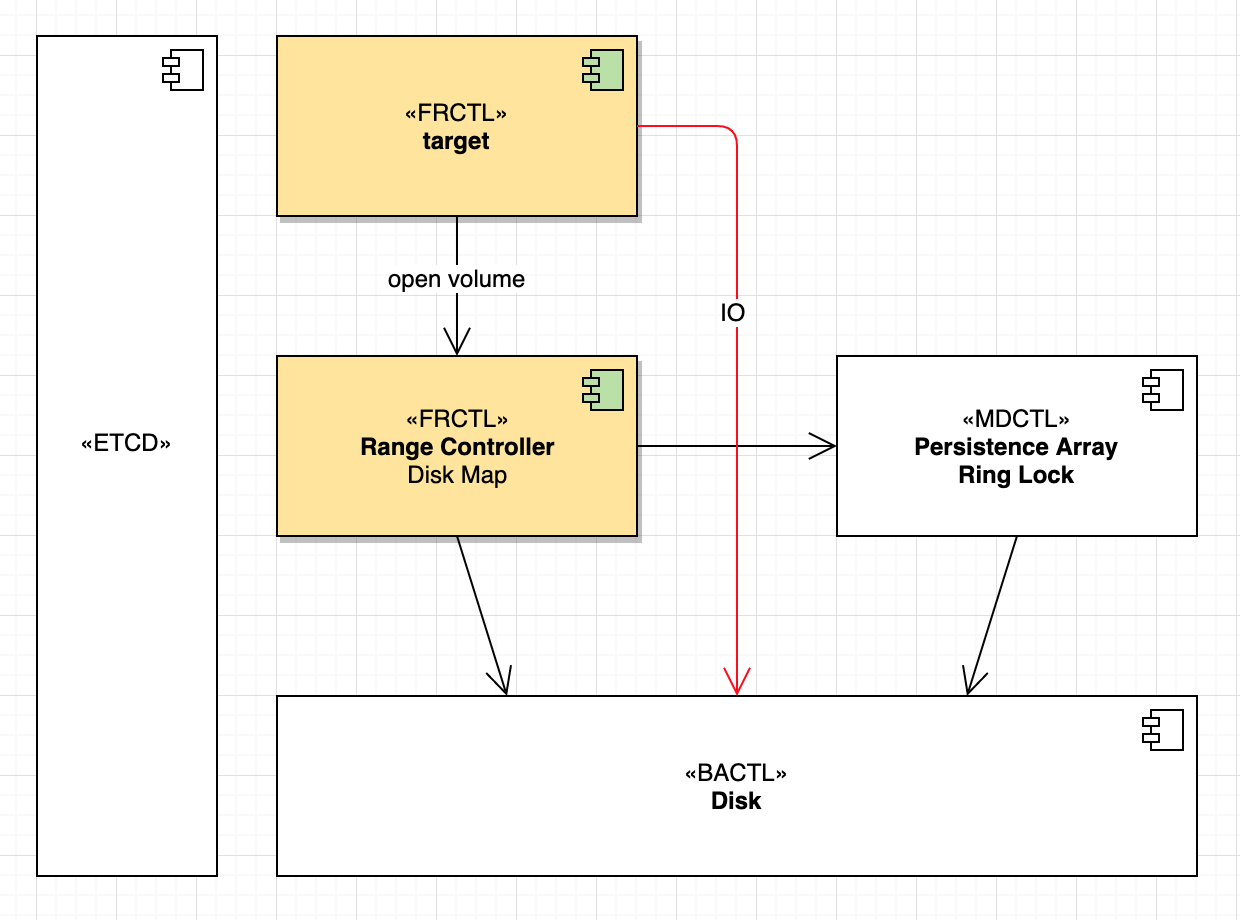
\includegraphics[width=0.9\textwidth]{../imgs/modules.png}
            \end{center}
        \end{column}

        \begin{column}{0.5\textwidth}
            \begin{center}
                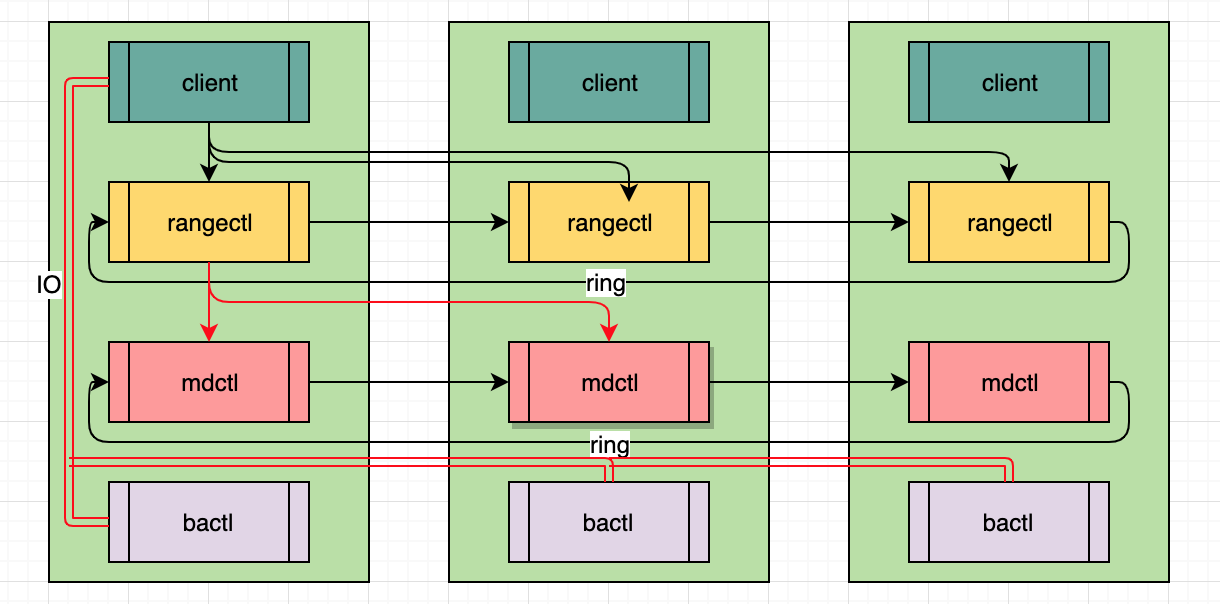
\includegraphics[width=0.9\textwidth]{../imgs/message-flow.png}
            \end{center}
        \end{column}
    \end{columns}

    \begin{myeasylist}{itemize}
        & Client
        & FrCtl (Target - VolumeCtl/RangeCtl)
        & MdCtl (无持久化)
        & BaCtl
        & ETCD
    \end{myeasylist}
\end{frame}

\begin{frame}[fragile]
    \frametitle{卷的地址空间}
    \begin{center}
        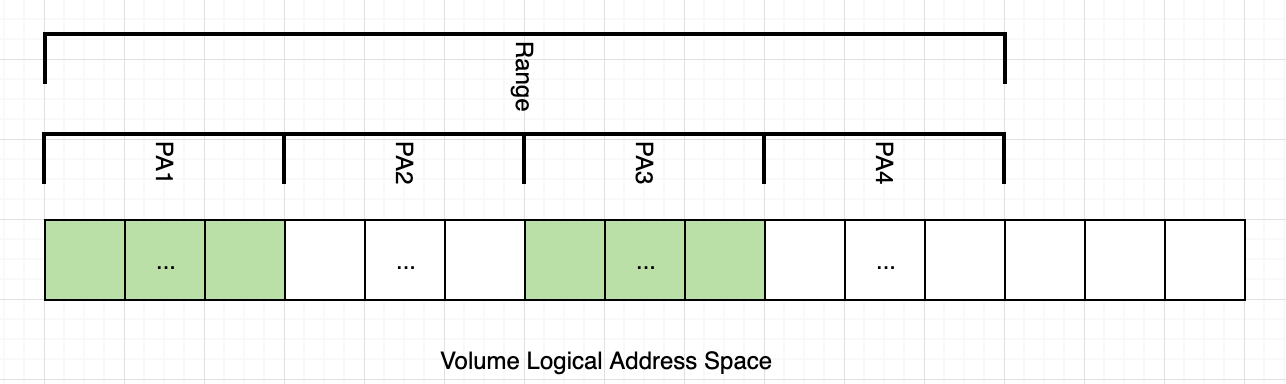
\includegraphics[width=0.9\textwidth]{../imgs/volume-addressspace.png}
    \end{center}

    \Activate
    \begin{tcolorbox}[title=分段管理]
        \begin{easylist}[itemize]
            & 一个卷包含若干range
            & 一个range包含4个Persistence Array(4M)
            & 一个Persistence Array包含若干chunk(4M)
            & 估算卷的最大大小:4M/128 x 4M/128 x 4M = 4PB
        \end{easylist}
    \end{tcolorbox}
    \Deactivate
\end{frame}

\begin{frame}
    \frametitle{卷的元数据}
    \begin{center}
        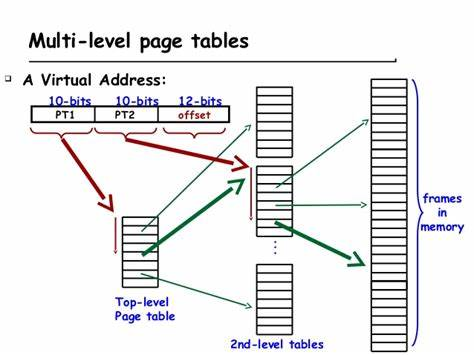
\includegraphics[width=0.6\textwidth]{../imgs/pagetable.jpeg}
    \end{center}
\end{frame}

\begin{frame}
    \frametitle{IO路径}
    \begin{center}
        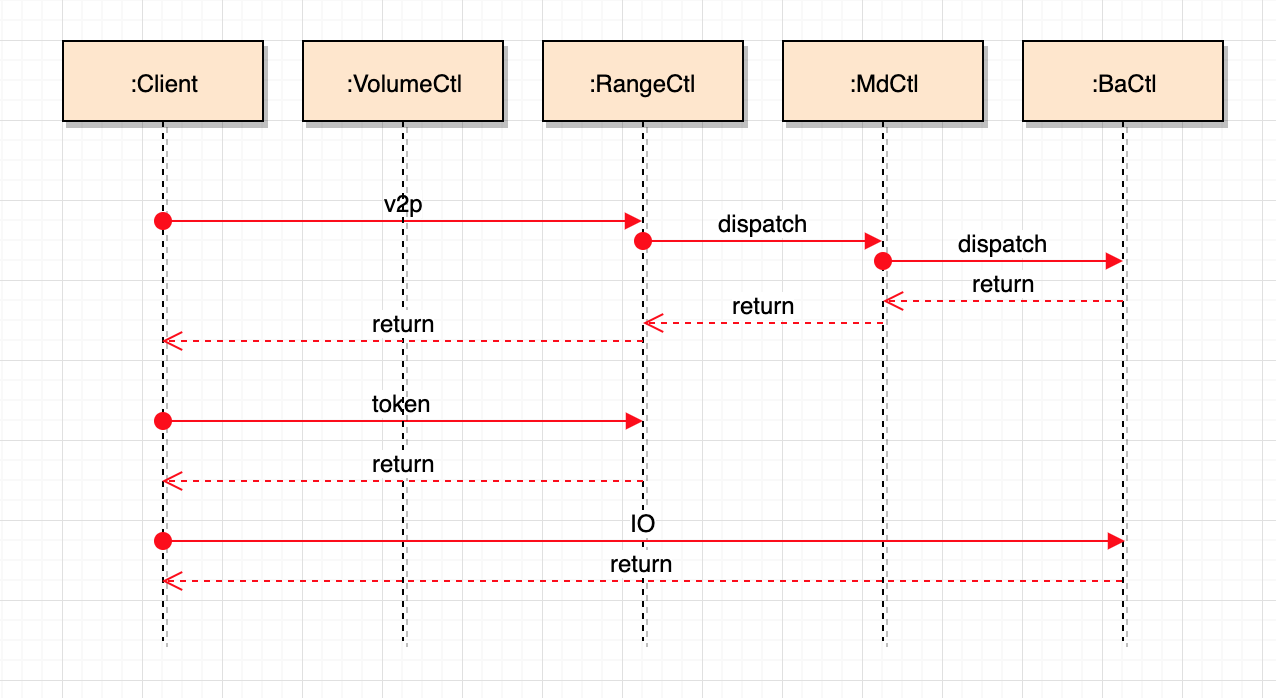
\includegraphics[width=0.9\textwidth]{../imgs/data-path.png}
    \end{center}
\end{frame}

\section{性能}

\begin{frame}[fragile]
    % \frametitle{水利工程}
    \begin{center}
        \includegraphics[width=0.8\textwidth]{../imgs/dujiangyan.jpg}
    \end{center}
\end{frame}

\subsection{起点}

\begin{frame}[fragile]
    \frametitle{0610 起点}
    \begin{myeasylist}{itemize}
        & 多进程
        & get\_token
        & 网络连接模型(all to all)
    \end{myeasylist}

    \begin{myeasylist}{itemize}
        & 1/1配置,fio,6w iops,AIO/TCP,iSCSI
    \end{myeasylist}
\end{frame}

\subsection{单卷}

\begin{frame}[fragile]
    \frametitle{0702}
    \begin{myeasylist}{itemize}
        & 完成所需内存管理模块(hugepage-based)
        & 对接libnvme,支持nvme驱动
        & 对接SPDK/NVMf,支持NVMf target
    \end{myeasylist}

    \begin{myeasylist}{itemize}
        & 1/1配置,fio,6w iops,对比AIO/TCP,性能无任何提升
    \end{myeasylist}
\end{frame}

\begin{frame}[fragile]
    \frametitle{0702 尝试各种优化项}
    \begin{columns}
        \begin{column}{0.5\textwidth}
            \begin{center}
                \includegraphics[width=0.8\textwidth]{../imgs/step1-1.png}
            \end{center}
        \end{column}
        \begin{column}{0.5\textwidth}
            \begin{center}
                \includegraphics[width=0.8\textwidth]{../imgs/step1-2.png}
            \end{center}
        \end{column}
    \end{columns}
    \begin{myeasylist}{itemize}
        & 移除频次高的LOG
        & O3
        & 关闭performance\_analysis特性
        & 分支预测
        & IO FUNC(io路径上的代码放入同一代码块,优化CPU cache)
    \end{myeasylist}
\end{frame}

\subsection{FRCTL}

\begin{frame}[fragile]
    \frametitle{0703 定位瓶颈在frctl?}
    \begin{myeasylist}{itemize}
        & 解析iSCSI target的协议
        & 主导rangectl和bactl的消息交互
        & frctl占用一个polling core,如果一个调度周期需要5us,则最高iops是20w。
        & 能解释迄今为止观测到的性能数据
            && AIO -> NVMe 无效
            && TCP -> RDMA 无效
            && 单卷多核,性能同单卷单核
        & \hl{如何优化frctl的调度能力成了首要问题}?
    \end{myeasylist}
\end{frame}

\begin{frame}[fragile]
    \frametitle{0703 优化frctl}
    \begin{myeasylist}{itemize}
        & variable管理(利用到TLS,放到core上
        & gettime (精度不够,开启后影响大)
        & hugepage(tiny\_mem, task stack)
        & inline
        & 分支预测
        & cpu cache miss
        & IO路径?
    \end{myeasylist}

    \begin{myeasylist}{itemize}
        & 通过perf top/stat分析热点函数
    \end{myeasylist}
\end{frame}

\begin{frame}[fragile]
    \frametitle{单卷性能到此为止?}
    \begin{center}
        \includegraphics[width=0.8\textwidth]{../imgs/step2-1.png}
    \end{center}
\end{frame}

\subsection{扩展}

\begin{frame}[fragile]
    \frametitle{0708}
    \begin{center}
        \includegraphics[width=0.8\textwidth]{../imgs/step3-1.png}
    \end{center}
\end{frame}

\begin{frame}[fragile]
    \frametitle{0708}
    \begin{center}
        \includegraphics[width=0.8\textwidth]{../imgs/step3-2.png}
    \end{center}
\end{frame}

\subsection{通信}

\begin{frame}[fragile]
    \frametitle{0710}
    \begin{center}
        \includegraphics[width=0.8\textwidth]{../imgs/step3-3.png}
    \end{center}
\end{frame}

\begin{frame}[fragile]
    \frametitle{0711}
    \begin{center}
        \includegraphics[width=0.8\textwidth]{../imgs/step3-4.png}
    \end{center}
\end{frame}

\begin{frame}[fragile]
    \frametitle{0712}
    \begin{center}
        \includegraphics[width=0.8\textwidth]{../imgs/step3-5.png}
    \end{center}
\end{frame}

\begin{frame}[fragile]
    \frametitle{0718}
    \begin{center}
        \includegraphics[width=0.8\textwidth]{../imgs/step3-6.png}
    \end{center}
\end{frame}

\begin{frame}[fragile]
    \frametitle{0722 晴}
    \begin{center}
        \includegraphics[width=0.8\textwidth]{../imgs/step3-0722.png}
    \end{center}
\end{frame}

\subsection{TGTCTL}

\begin{frame}[fragile]
    \frametitle{0724}
    \begin{center}
        \includegraphics[width=0.8\textwidth]{../imgs/step3-0724.png}
    \end{center}
\end{frame}

\begin{frame}[fragile]
    \frametitle{0726}
    \begin{center}
        \includegraphics[width=0.8\textwidth]{../imgs/step3-0726.png}
    \end{center}
\end{frame}

\begin{frame}[fragile]
    \frametitle{怎么分析单卷性能?}
    \begin{center}
        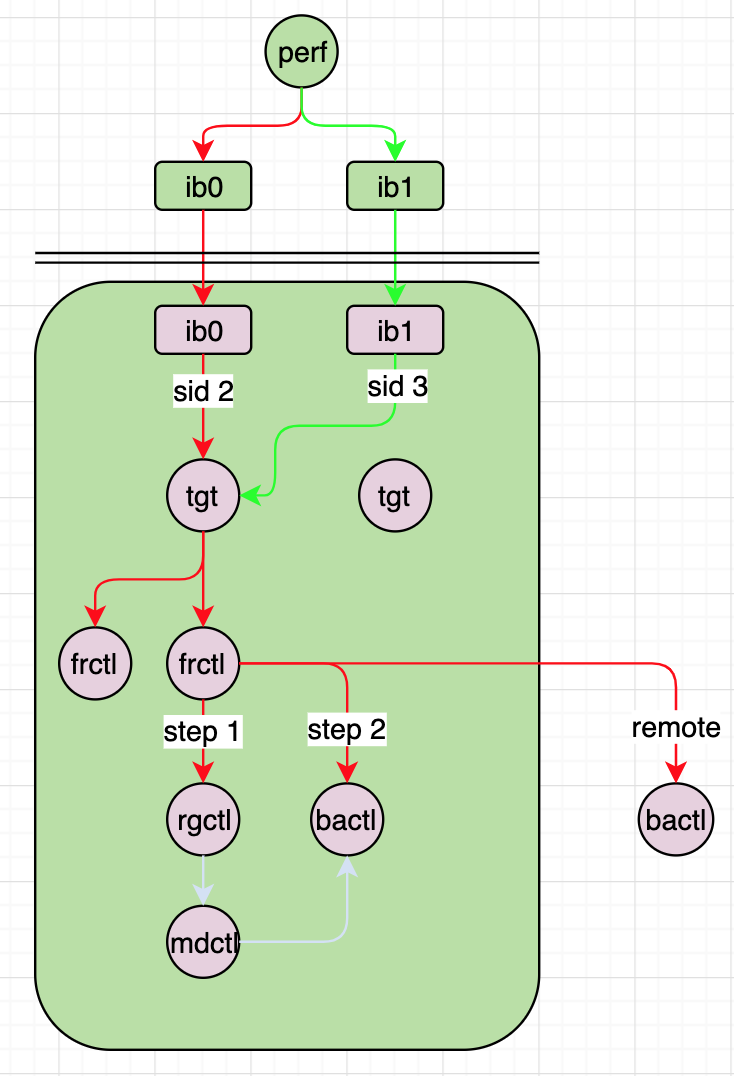
\includegraphics[width=0.4\textwidth]{../imgs/io-path.png}
    \end{center}
\end{frame}

\begin{frame}[fragile]
    \frametitle{多控架构}
    \begin{center}
        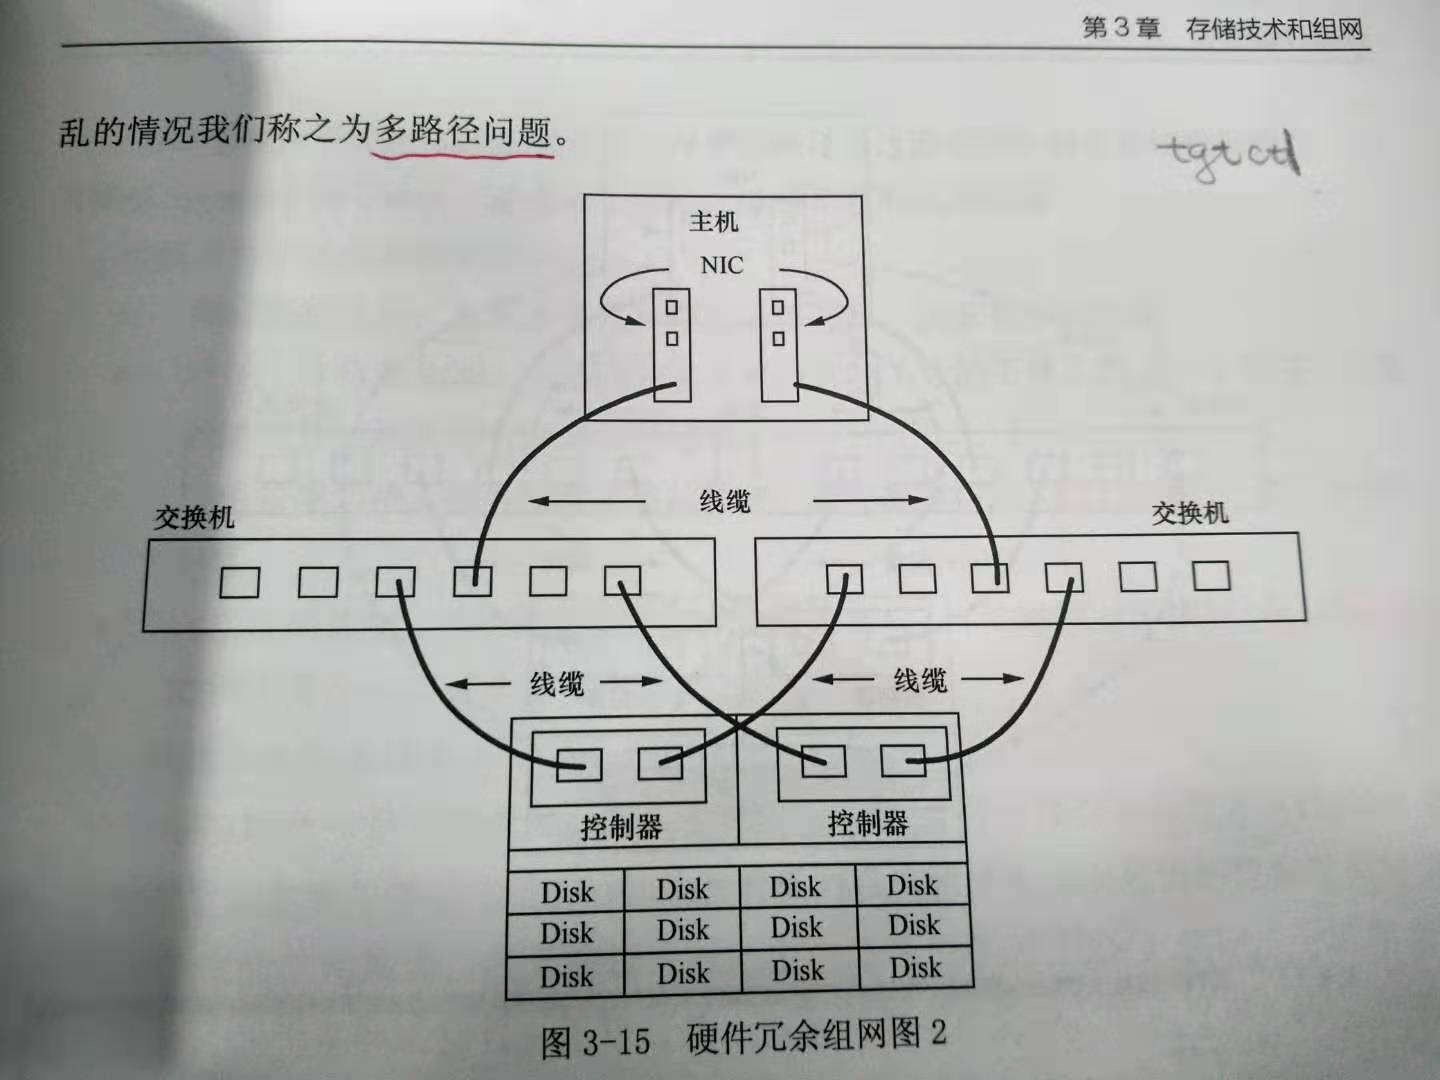
\includegraphics[width=0.6\textwidth]{../imgs/multipath-deployment.jpeg}
    \end{center}
\end{frame}

\begin{frame}[fragile]
    \frametitle{0806}
    \begin{center}
        \includegraphics[width=0.8\textwidth]{../imgs/step3-0806.png}
    \end{center}
\end{frame}

\begin{frame}[fragile]
    \frametitle{新起点、新征途}
    \begin{center}
        \includegraphics[width=0.8\textwidth]{../imgs/perf.jpeg}
    \end{center}
\end{frame}

\subsection{结论}

\begin{frame}[fragile]
    \frametitle{启示}
    \begin{myeasylist}{itemize}
        & 硬件
        & 架构对性能有巨大影响
            && 平衡
            && 局部性
            && 并行
            && 流水线
        & 模型
        & 工欲善其事必先利其器
            && trace (系统的可追踪性)
            && perf
            && Test Tool
    \end{myeasylist}
\end{frame}

\section{其它}

\begin{frame}[fragile]
    \frametitle{工具}
    \begin{center}
        \includegraphics[width=0.6\textwidth]{../imgs/tool.png}
    \end{center}
\end{frame}

\begin{frame}[fragile]
    \frametitle{平衡过程}
    \begin{center}
        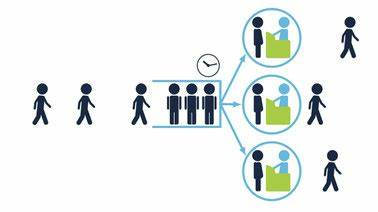
\includegraphics[width=0.6\textwidth]{../imgs/queuing.jpeg}
    \end{center}

    \begin{myeasylist}{itemize}
        & 流出量和流入量趋于平衡
        & 流入量 \ding{226} 调度能力 \ding{226} 处理能力
    \end{myeasylist}
\end{frame}

\begin{frame}[fragile]
    \frametitle{PDCA循环}
    \begin{center}
        \includegraphics[width=0.6\textwidth]{../imgs/PDCA.png}
    \end{center}
\end{frame}

%\begin{frame}[fragile]
%    \frametitle{一致性分割}
%    \begin{center}
%        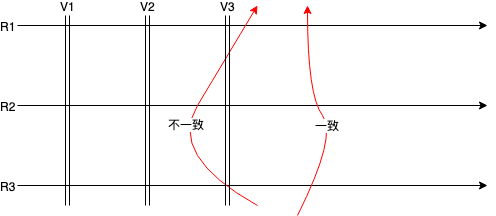
\includegraphics[width=0.6\textwidth]{../imgs/consistency-splice.png}
%    \end{center}

%    \begin{columns}
%        \begin{column}{0.5\textwidth}
%            \Activate
%            \begin{tcolorbox}[title=规定]
%                \begin{easylist}[itemize]
%                    & 更新一致性
%                    & 读取一致性
%                    & 副本一致性
%                    & EC一致性
%                \end{easylist}
%            \end{tcolorbox}
%            \Deactivate
%        \end{column}
%        \begin{column}{0.5\textwidth}
%            \Activate
%            \begin{tcolorbox}[title=实现]
%                \begin{easylist}[itemize]
%                    & Leader
%                    & Version
%                    & Journal
%                \end{easylist}
%            \end{tcolorbox}
%            \Deactivate
%        \end{column}
%    \end{columns}
%\end{frame}

\end{document}
